\section{Digital Interfaces}\label{sec:digital-interfaces}

	All sensoring data was obtained using analog channels, some digital channels will be reserved on the board in order to provide another type of sensing and control.

	\subsection{Digital Outputs}\label{ssec:digital-outputs}

		\subsubsection{Low-side Driver}\label{sssec:digital-outputs-low-side-driver}

			Item \ref{itm:func-req-11} from Section \ref{sec:functionalRequirements} states that the system must have a digital output channel to control a relay (check section \ref{ssec:relay}). According to \cite{songle-relay-datasheet}, a standard 5V (MCU operating voltage, Section \ref{ssec:the-choosen-mcu}) relay will have a nominal current of 89.3mA, the microcontroller's datasheet \cite{atmega328p-datasheet} says that the maximum DC current per I/O pin is 40mA though. Hence it is not possible to activate a relay connected directly to a MCU's I/O pin.
			\par 
			In order to solve this a relay driver circuit needs to be used, in this case a low side mosfet driver similar to the one from Figure \cite{pmos-low-side-driver} will be used.

			\begin{figure}[htbp]
				\centering
				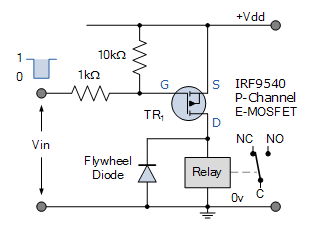
\includegraphics[scale=1]{figuras/fig-pmos-low-side-driver.png}
				\caption{PMOS low side driver \cite{pmos-low-side-driver}}
				\label{fig:pmos-low-side-driver}
			\end{figure}

			This is a low-side driver, when the PMOS is submitted to a high logic level (5V) in it's gate it will enter on the cutoff region and will not conduct current, hence not activating the relay. On the other hand, when a low logic level (0V) is applied to the device's gate it will enter the saturation region and will conduct current, hence activating the relay (check Section \ref{ssec:mosfet}).

		\subsubsection{Digital Output Circuit}\label{sssec:digital-output-circuit}

			The digital output circuit will be very similar to the one from Figure \ref{fig:pmos-low-side-driver}. The power supply connected to the mosfet will be the 12V source (check Section \ref{sssec:12v-supply}), on the PMOS drain there will be a TVS diode (check Section \ref{sssec:tvsTransientProtection}) with a standoff voltage of 12V (SMBJ12A from \textit{Littlefuse} \cite{smbj12a-datasheet}, this TVS will protect the PMOS from reverse current and from overvoltages. Using 12V instead of 5V provides lower current and by Ohm's Law the voltage drop is proportional to the current flowing through a load. So increasing this voltage can ensure that the voltage drop during the connection to the relay will be lower. Figure \ref{fig:digital-output-circuit} show the equivalent circuit for the digital output.

			\begin{figure}[htbp]
				\centering
				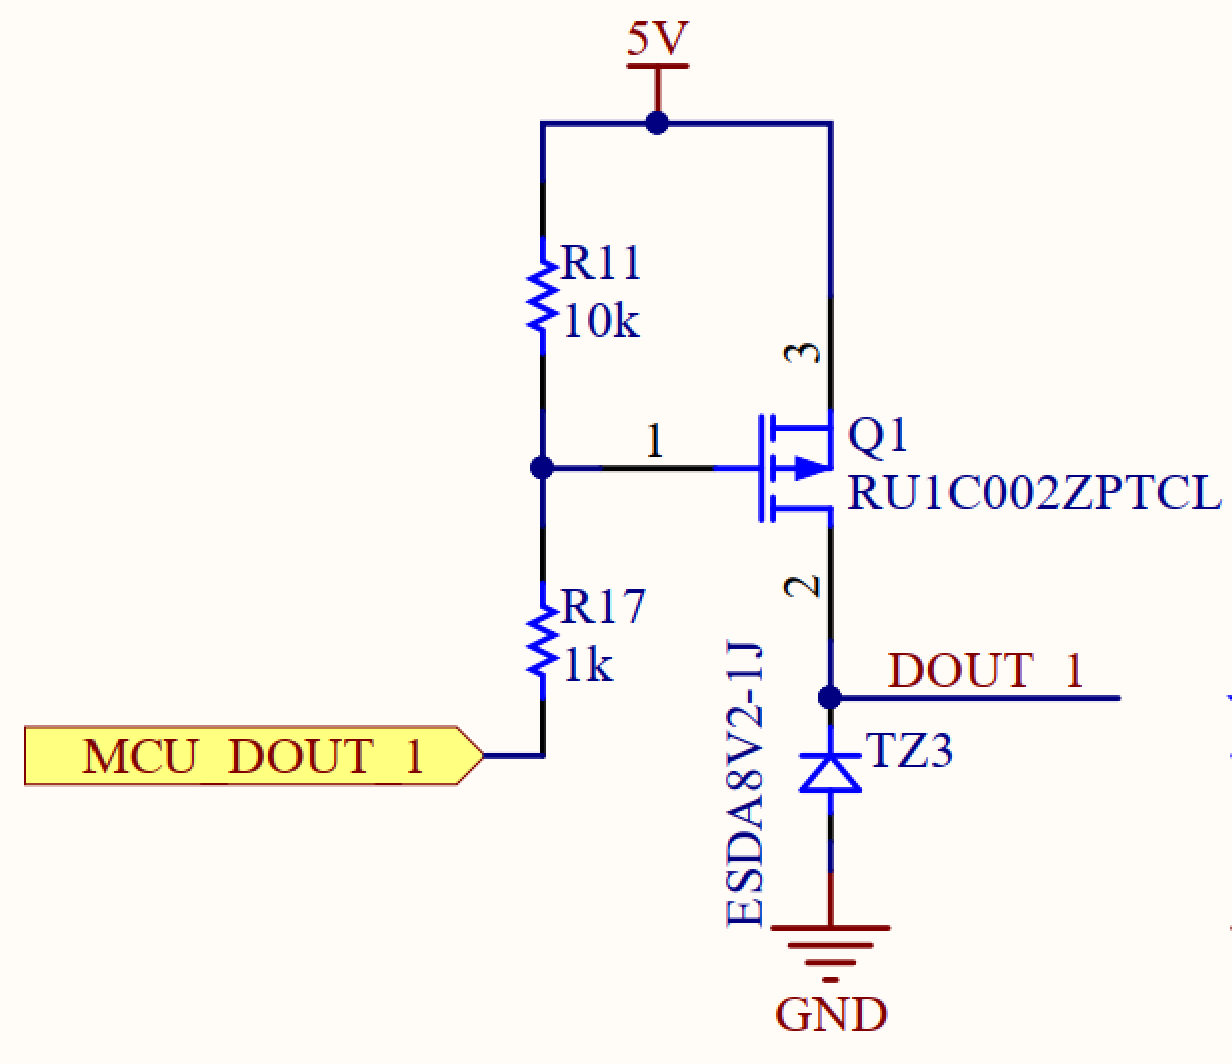
\includegraphics[scale=1]{figuras/fig-digital-output-circuit.png}
				\caption{Digital Output Circuit \cite{digital-output-circuit}}
				\label{fig:digital-output-circuit}
			\end{figure}

			The selected PMOS is the NDS332P from \textit{Fairchild} \cite{nds332p-datasheet}, it has a maximum operating continuos current of 1A, maximum gate threshold voltage of 1V, maximum drain-source voltage of 20V and maximum gate source voltage of $\pm$8V. It is adequate for this purpose. Resistor R4 is used to limit the magnitude of the current spike that can occur when a driver switches fast and has to charge or discharge a large gate capacitance. Resistor R7 is a pull-up for the gate, it will ensure that the PMOS will be in cutoff region if there is no input for the MCU. Resistor R10 is optional, for activating relays it is not needed, but other loads may require a pull-down, that is why it was placed on the PMOS drain. It was decided to keep any relay out of the board to save space. Moreover, keeping the relay out of the board gives room for using this digital output for other purposes. Fuse F2 is used to limit the current on the TVS in a scenario in which the TVS reaches it`s clamping voltage.

	\subsection{Digital Inputs}\label{ssec:digital-inputs}

		This project does not have any requirement for digital inputs. However, in order to make the project more versatile for the future, it was decided to keep the space on the layout for soldering components to implement digital inputs. Figure \ref{fig:digital-input-circuit} show the circuit to interface the digital inputs.

			\begin{figure}[htbp]
				\centering
				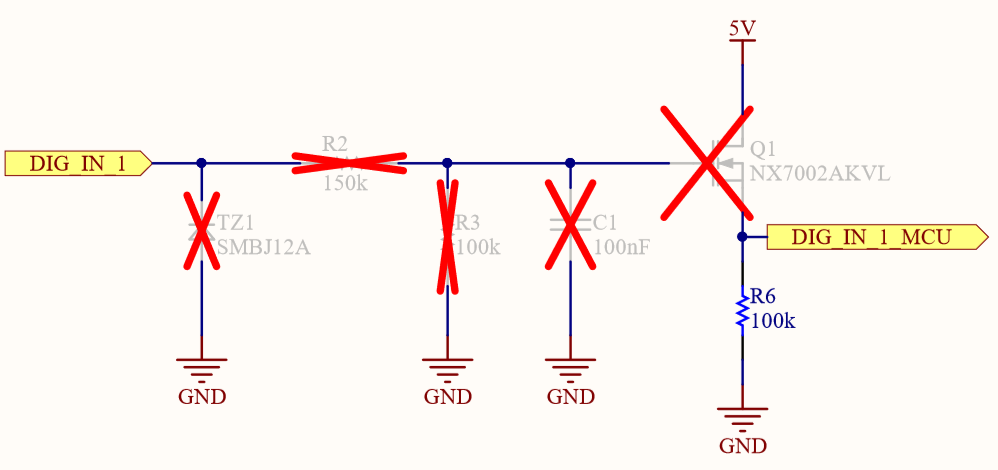
\includegraphics[scale=1]{figuras/fig-digital-input-circuit.png}
				\caption{Digital Input Circuit \cite{digital-input-circuit}}
				\label{fig:digital-input-circuit}
			\end{figure}

		The choosen NMOS was the NX7002AK from \textit{Nexperia} \cite{nx7002ak-datasheet}.This is a extremely versatile NMOS, it has a maximum drain source voltage of 60V, maximum gate-source voltage of $\pm$20V and maximum drain current of 300mA. This circuit is basically a buffer, it is used just to convert the state of the input signal to the MCU voltage limits. 

		This circuit is adjustable to different input voltages ($V_{IN}$), R2 and R3 creates a voltage divider and must be choosen according to Equation \ref{eqn:voltage-divider-digital-input}.

		\begin{equation}\label{eqn:voltage-divider-digital-input}
			2.1 < \frac{R3}{R2 + R3} \cdot V_{IN} < 5V
		\end{equation}

		For a 12V voltage input as an example, using $R_{2}=150k\omega$ and $R_{3}=100k\omega$ will produce a voltage at the gate equal to 4.8V, meeting the limits from Equation \ref{eqn:voltage-divider-digital-input}.

		This circuit also has a LPF formed by the combination of R2 and C1, it is used to filter any noise from the input. Equation \ref{eqn:1st-order-lpf-fc} is used to calculate the center frequency of this filter.

		\begin{equation}\label{eqn:1st-order-lpf-fc}
			f_{C} = \frac{1}{2 \cdot \pi \cdot R2 \cdot C1}
		\end{equation}

		The center frequency $f_{C}$ must be greater than the maximum input signal frequency to ensure operation.

		Finally, TZ1 is a TVS diode, it must be a TVS diode with a standoff voltage equal to the maximum input voltage. The layout was made to fit a SMBJ12CA from \textit{Littlefuse} \cite{smbj12a-datasheet}, this device has the DO-214AB, any device with the same footprint can be soldered on it's pads.
